\documentclass[crop,tikz]{standalone}
\usetikzlibrary{%
    arrows,
    arrows.meta,
    backgrounds,
    calc,
    decorations.pathreplacing,
    fit,
    matrix,
    positioning,
    scopes,
    shadows
}
\usepackage[charter]{mathdesign}

\begin{document}
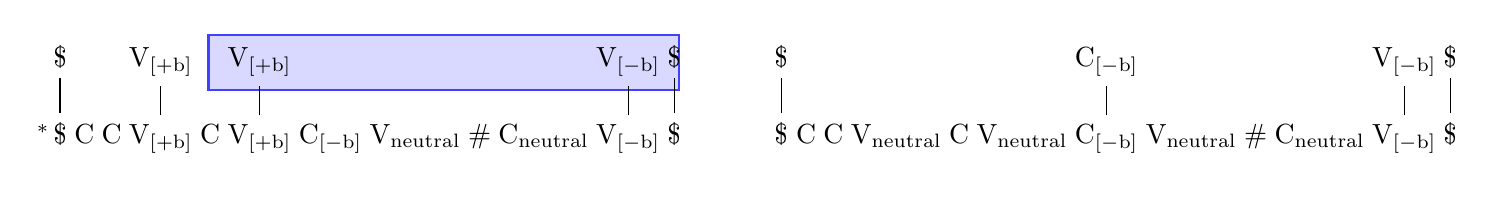
\begin{tikzpicture}
    \matrix (bad)  [matrix of nodes, ampersand replacement=\&,
                    column sep=-.4em, row sep=1em,
                   ] {
        \$ \&   \&   \& V$_\mathrm{[+b]}$ \&   \& V$_\mathrm{[+b]}$ \&                   \&                      \&    \&                      \& V$_\mathrm{[-b]}$ \& \$\\
        %
        \$ \& C \& C \& V$_\mathrm{[+b]}$ \& C \& V$_\mathrm{[+b]}$ \& C$_\mathrm{[-b]}$ \& V$_\mathrm{neutral}$ \& \# \& C$_\mathrm{neutral}$ \& V$_\mathrm{[-b]}$ \& \$\\
    };
    \node at (bad-2-1.west) {$^*$};

    \matrix (good) [matrix of nodes, ampersand replacement=\&,
                    column sep=-.4em, row sep=1em,
                    right=2em of bad
                   ] {
        \$ \&   \&   \&                      \&   \&                      \& C$_\mathrm{[-b]}$ \&                      \&    \&                      \& V$_\mathrm{[-b]}$ \& \$\\
        %
        \$ \& C \& C \& V$_\mathrm{neutral}$ \& C \& V$_\mathrm{neutral}$ \& C$_\mathrm{[-b]}$ \& V$_\mathrm{neutral}$ \& \# \& C$_\mathrm{neutral}$ \& V$_\mathrm{[-b]}$ \& \$\\
    };

    \foreach \Node in {1,4,6,11,12}
        \draw (bad-1-\Node) to (bad-2-\Node);
    \foreach \Node in {1,7,11,12}
        \draw (good-1-\Node) to (good-2-\Node);

    \begin{pgfonlayer}{background}
        \foreach \Matrix/\Start/\End in {%
            bad/6/11%
            }
            \node[draw,blue!75,fill=blue!15,thick,
                  minimum height=2em, anchor=south,
                  fit=(\Matrix-1-\Start.west)(\Matrix-1-\End.east)
                 ]
                  {};
    \end{pgfonlayer}
\end{tikzpicture}
\end{document}
